% UTF-8

\documentclass[../main/thesis.tex]{subfiles}
\begin{document}



%\newpage\addcontentsline{toc}{chapter}{Aufgabenstellung}
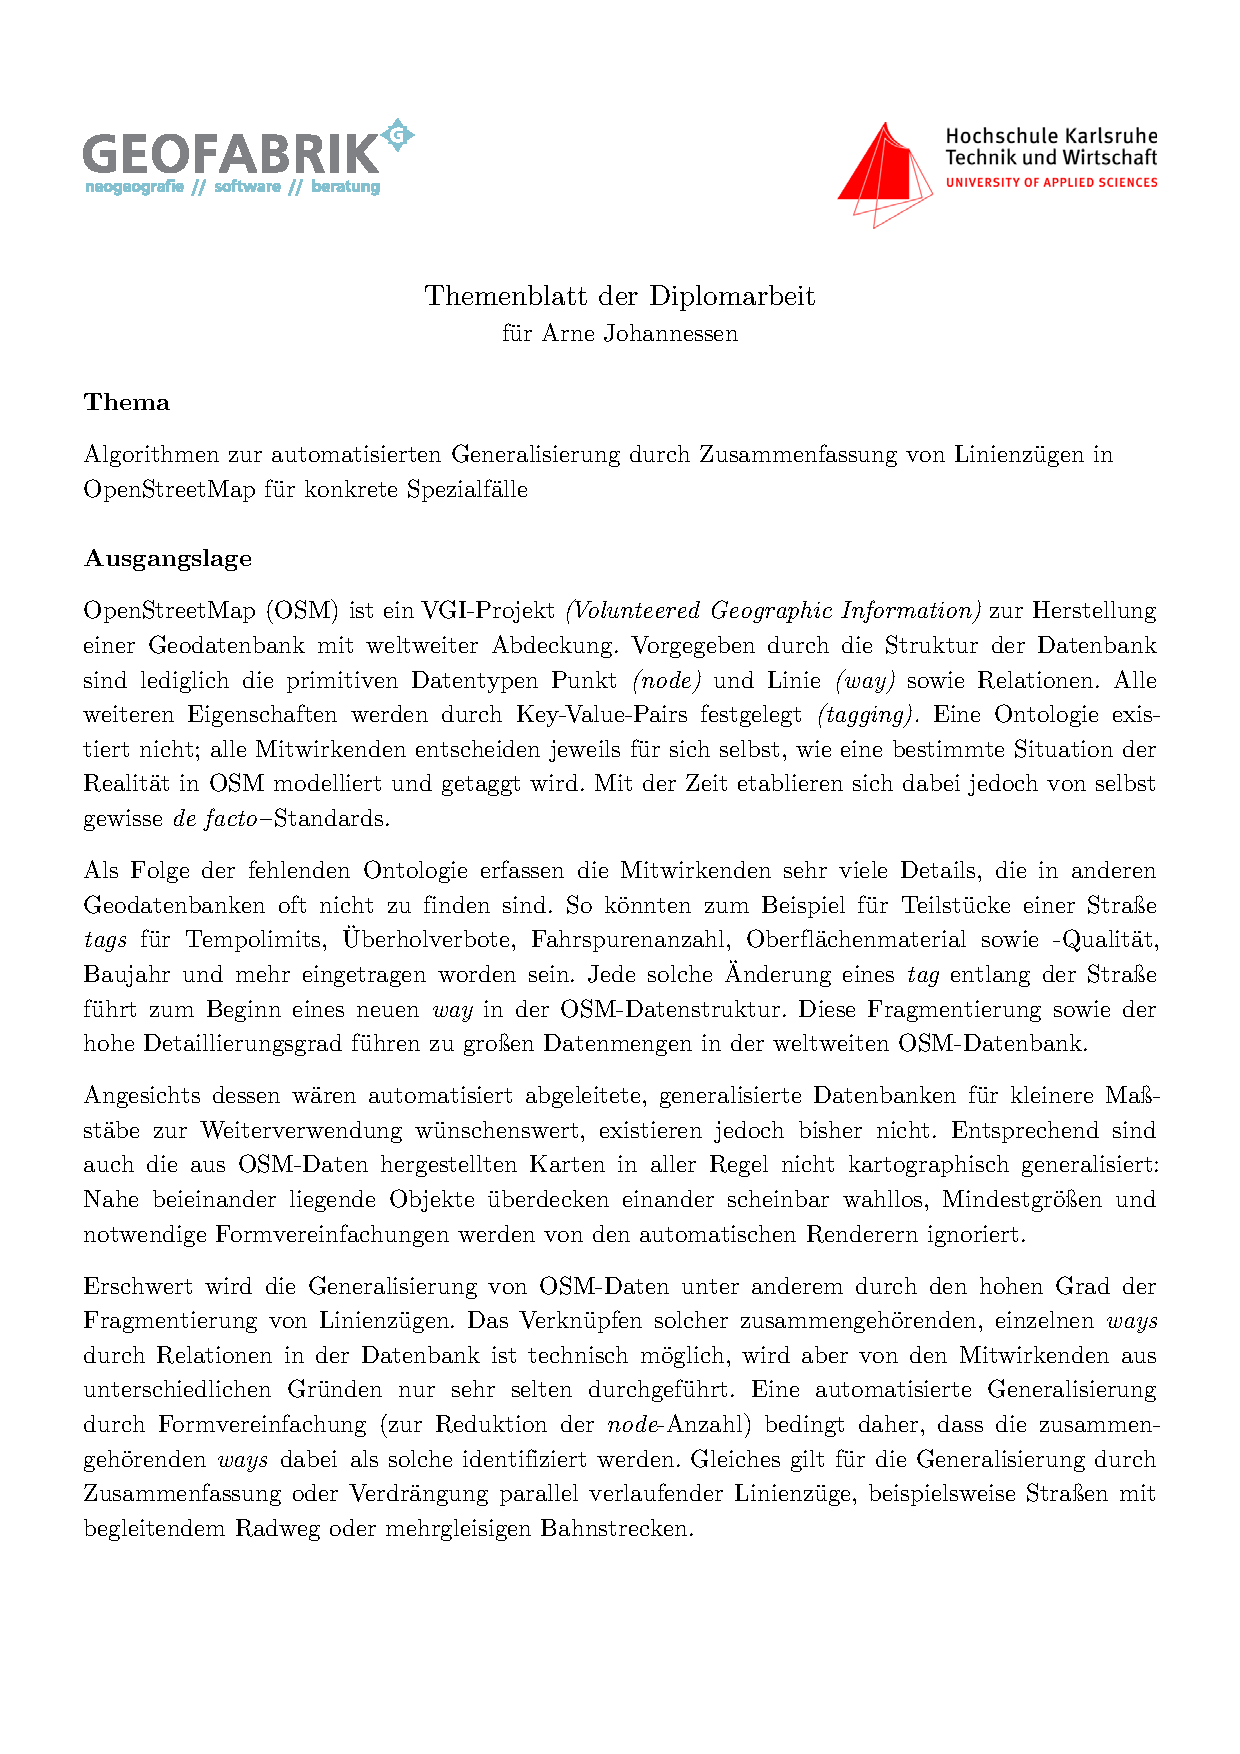
\includepdf[pages={-},noautoscale=true,scale=.85]{../main/Themenblatt}



\chapter*{Vorbemerkung}
\thispagestyle{empty}

Wie in der Aufgabenstellung auf der vorangehenden Seite ersichtlich, war die vorliegende Diplomarbeit bereits Ende~2012 ausgegeben worden.
Sie sollte ursprünglich im April~2013 fertiggestellt werden.
Aufgrund sehr langer krankheitsbedingter deutlicher Einschränkungen der Arbeitsfähigkeit des Verfassers konnte sie -- mit Genehmigung des zuständigen Prüfungsausschusses -- erst bedeutend später abgeschlossen werden.

Die Arbeit vollständig auf den heutigen Stand zu aktualisieren, hätte eine Neubearbeitung wesentlicher Teile erfordert.
Die damit einhergehende zusätzliche Zeitverzögerung hätte die Vergleichbarkeit mit anderen Abschlussarbeiten weiter verschlechtert.
Um dies zu vermeiden, entspricht diese Diplomarbeit in den wesentlichen Punkten -- mit dem Einverständnis der Betreuer -- dem Stand der Wissenschaft im Jahr 2013.

% (überdies verschobener Fokus, mehr hin zu Technik als erwartet)

Einige Kartenausschnitte sind neueren Datums; dies ist jeweils anhand der Quellenangabe ersichtlich.
Weitere neuere Aspekte sind -- soweit möglich -- entweder in Fußnoten ergänzt oder abschließend in Abschnitt~\ref{ch:recent-research} „\nameref{ch:recent-research}“ (Seite~\pageref{ch:recent-research}) berücksichtigt.

\vspace{1em}

\noindent \textit{Arne Johannessen, im Februar~2018}



\end{document}
